\documentclass[11pt, A4paper]{article}

\usepackage[a4paper, left=2cm, right=2cm, top=2cm]{geometry}
\usepackage{amsmath}
\usepackage{amsfonts}
\usepackage{amssymb}
\usepackage[english]{babel}
\usepackage{graphicx}
\usepackage[T1]{fontenc}
\usepackage{listings}
\usepackage[dvipsnames]{xcolor}
\usepackage[font=small,labelfont=bf]{caption}
\usepackage{etoolbox}
\usepackage{subcaption}
\usepackage{braket}
\usepackage{mathtools}
\usepackage{graphicx}
\usepackage{caption}



\usepackage{soul}

\newcommand{\blue}[1]{\colorbox{SkyBlue}{#1}}
\newcommand{\yell}[1]{\colorbox{Yellow}{#1}}
\newcommand{\numpy}{\texttt{numpy}}
\newcommand{\dt}[1]{{\text{d} \over \text{dt} }\braket{#1}}
\newcommand{\dtt}[1]{{\text{d}^2 \over \text{dt}^2 }\braket{#1}}
\newcommand{\pt}[1]{{\partial \over \partial #1}}
\newcommand{\ptt}[1]{{\partial^2 \over \partial #1 ^2}}
\newcommand{\br}[1]{\braket{\hat{#1}}}
\newcommand{\brs}[1]{\braket{\hat{#1}^2}}
%\renewcommand{\hat}{}
\newcommand{\comu}[2]{\braket{[#1,#2]}}
\definecolor{codegreen}{rgb}{0,0.6,0}
\definecolor{codegray}{rgb}{0.5,0.5,0.5}
\definecolor{codepurple}{rgb}{0.58,0,0.82}
\definecolor{backcolour}{rgb}{0.95,0.95,0.92}

\lstdefinestyle{mystyle}{
    backgroundcolor=\color{backcolour},   
    commentstyle=\color{codegray},
    keywordstyle=\color{magenta},
    numberstyle=\tiny\color{codegray},
    stringstyle=\color{codepurple},
    basicstyle=\ttfamily\footnotesize,
    breakatwhitespace=false,         
    breaklines=true,                 
    captionpos=b,                    
    keepspaces=true,                 
    numbers=left,                    
    numbersep=5pt,                  
    showspaces=false,                
    showstringspaces=false,
    showtabs=false,                  
    tabsize=2
}

\lstset{style=mystyle}
\newcommand{\SG}{Schr\"odinger }
\newcommand{\N}{\mathbb{N}}
\newcommand{\refEq}[1]{eq.(\ref{#1})}
\newcommand{\refList}[1]{listing(\ref{#1})}
\newcommand{\refFig}[1]{fig.(\ref{#1})}
\newcommand{\T}[1]{\texttt{#1}}
\newcommand{\Int}[1]{\int _{-\infty}^{\infty} #1\text{d}x}
\makeatletter
\def\@seccntformat#1{\@ifundefined{#1@cntformat}%
   {\csname the#1\endcsname\quad}  % default
   {\csname #1@cntformat\endcsname}% enable individual control
}
\let\oldappendix\appendix %% save current definition of \appendix
\renewcommand\appendix{%
    \oldappendix
    \newcommand{\section@cntformat}{\appendixname~\thesection\quad}
}
\makeatother


\makeatletter
\patchcmd{\maketitle}{\@fnsymbol}{\@arabic}{}{}
\makeatother

\title{Computational Physics Exam: \\ Quantum Harmonic Oscillator}
\author{Tamilarasan Ketheeswaran 411069\footnote{tamilarasan.ketheswaran@rwth-aachen.de}}
\date{28 July 2023}



\begin{document}


\maketitle
\tableofcontents

\section{Introduction}
In this exam, we deal with the simulation of the quantum harmonic oscillator. First, we find an analytic expression for the averages and variances of the position of a wavepacket in such a potential, after which we discuss the simulation method we use to do a numerical calculation of the values. Consequently, we present the results and compare them to the analytical expression. 

For the simulation, we use the programming language \T{Python} and the packages \T{numpy}\footnote{abbreviated as \T{np}} and to plot our results \T{matplotlib}. Moreover, from \T{numba} we import \T{njit} and from \T{multiprocessing} \T{Pool} for a faster simulation. \\
\clearpage
\section{Theoretical Framework}
\label{sec: theo}
In this section, we govern the theory behind the system. Having a particle in a harmonic potential, we are interested in the time evolution of the particle's mean position $\braket{x(t)}$ and variance $\text{Var}(x(t))$.
Setting $m = 1$ and $\hbar = 1$, the \SG equation in position space for a harmonic potential is given by
\begin{align}
	i\pt{t} \Phi(x,t) &= \left(-{1\over 2} \ptt{x} + {\Omega ^2 \over 2} x^2\right)  \Phi(x,t) \label{eq: SG}\\
	\intertext{Or in a more general description, by}
	\hat{H}\ket{\Phi(t)} &= \left({\hat{p}^2\over 2} + {\Omega ^2 \over 2} \hat{x}^2 \right) \ket{\Phi(t)}.
	\label{eq: SG gen}
\end{align}
Initially, at $t=0$, the wavepacket is described via
\begin{equation}
	\braket{x |\Phi(t)} = \Phi (x, t = 0) = \Phi _0= \left({1\over {\sqrt{\pi \sigma^2}}}\right)^{1\over 2}e^{-{(x-x_0)^2 \over 2\sigma^2}},
	\label{eq: initial}
\end{equation}
a gaussian wavepacket of width ${\sigma\over\sqrt{2}}$ centered around $x_0$.
We focus ourselves on the calculation of $\braket{x(t)}$ and $\braket{x^2(t)}$. For that, we make use of the \textit{Ehrenfest Theorem}:
\begin{equation}
	\dt{\hat{O}} = {1 \over i} \comu{\hat{O}}{\hat{H}} +\left\langle{ \partial \hat{O} \over \partial t}\right\rangle.
	\label{eq: ET}
\end{equation}
The position operator $\hat{x}$ and momentum operator $\hat{p}$ do not depend on time, such that the derivative on the RHS vanishes.
In general, the average of an operator $\braket{O}$ can be calculated using
\begin{equation}
	\braket{O} = \braket{\Phi(t)|\hat{O}|\Phi(t)} =\Int{\Phi ^*(x,t) O \Phi(x,t)}.
	\label{eq: scalar}
\end{equation}
In the following derivation, we make use of the three commutator relations
\begin{equation}
	[\hat{x},\hat{p}] = i, \qquad 	[\hat{x},\hat{p}^2] = 2i\hat{p}, \qquad 	[\hat{x}^2,\hat{p}] = 2i\hat{x}, 
\end{equation}
and the fact that $[\hat{x},\hat{x}] = [\hat{p},\hat{p}] = 0$.
Starting with the Ehrenfest theorem for both the position and momentum operator, with our definition for $\hat{H}$ from \refEq{eq: SG gen}, we obtain
\begin{align}
	\dt{\hat{x}} &= {1 \over i} \comu{\hat{x}}{\hat{H}} = {1\over 2i} \braket{[\hat{x},\hat{p}^2]} = \braket{\hat{p}} \label{eq: dtx = p}\\
	\intertext{and}
	\dt{\hat{p}} &= {1 \over i} \comu{\hat{p}}{\hat{H}} = {\Omega ^2\over 2i} \braket{[\hat{p},\hat{x}^2]} = - \Omega ^2\braket{\hat{x}}. \\
	\intertext{Taking another time derivative of $\dt{\hat{x}}$, we have} 
	\dtt{\hat{x}}&= \dt{\hat{p}} \qquad \Rightarrow \qquad \dtt{\hat{x}} = - \Omega ^2\braket{\hat{x}}.
\end{align}
The second-order differential equation above can be solved with the ansatz
\begin{align*}
	&\braket{x(t)} = +A\cos(\Omega t) + B\sin(\Omega t)\\
		\text{from \refEq{eq: dtx = p}}\Rightarrow &\braket{p(t)} = -A\Omega\sin(\Omega t) + B\Omega\cos(\Omega t).
\end{align*}
According to \refEq{eq: scalar}, the mean initial position $\braket{x}|_{t=0}$ and momentum $\braket{p}|_{t=0}$ is, 
\begin{align*}
	\braket{x(t)}\Big|_{t=0} & = \Int{x|\Phi _0|^2} = x_0\\
	\braket{p(t)}\Big|_{t=0} & = \Int{\Phi _0^* {1\over i }\pt{x}\Phi _0 } = 0.
\end{align*}
With these initial conditions, we have conditions governing $A$ and $B$.
Inserting them into our ansatz, we are left with
\begin{align*}
	&\braket{x(0)} = A = x_0 \quad \text{and} \quad \braket{p(0)} =  B\Omega= 0,
\end{align*}
such that
\begin{equation}
	\braket{x(t)} = x_0 \cos(\Omega t).
	\label{eq: x sol}
\end{equation}


Now, we dedicate ourselves to the calculation of $\braket{x^2(t)}$. Again, from the Ehrenfest theorem in \refEq{eq: ET}
\begin{align}
	\dt{\hat{x}^2} &= {1\over i}\comu{\hat{x}^2}{\hat{H}} = {1\over 2 i}\comu{\hat{x}^2}{\hat{p}^2} = \braket{\hat{x}\hat{p}+\hat{p}\hat{x}} =2 \braket{\hat{x}\hat{p}} -i \label{eq: dtxx}\\
	\dt{\hat{x}\hat{p}} &= {1\over i}\comu{\hat{x}\hat{p}}{\hat{H}} = {1\over i}\braket{\hat{x}[\hat{p},\hat{H}]+[\hat{x},\hat{H}]\hat{p}} = \braket{\hat{p}^2}- \Omega ^2\braket{\hat{x}^2}.
	\label{eq: dtxp}
\end{align}
To obtain a term for $\brs{p}$, we use the 
\begin{align}
\text{from \refEq{eq: SG gen}}	\Rightarrow \br{H} &= {\brs{p} \over 2} + {\Omega^2 \over 2} \brs{x}\nonumber \\
	\Leftrightarrow \brs{p} &= 2\br{H} -\Omega^2 \brs{x},\nonumber
\end{align}
such that \refEq{eq: dtxp} changes to
\begin{align}
	\dt{\hat{x}\hat{p}} &= 2\br{H}- 2\Omega ^2\braket{\hat{x}^2}. \label{eq: dt xp = 2H}\\
	\intertext{After taking another time derivative of the term in \refEq{eq: dtxx}, we insert the \refEq{eq: dt xp = 2H}, such that}
	\dtt{\hat{x}^2} &=  4\br{H}- 4\Omega ^2\braket{\hat{x}^2} \nonumber\\
	&= {4\Omega ^2}\left({\br{H}\over \Omega ^2} -\brs{x} \right).\label{eq: ddxx = eq}
\intertext{With no explicit time dependence in the Hamiltonian (see \refEq{eq: SG gen}), we deduct the total conservation of the energy of the system, which is why $ \br{H} = \braket{H(t=0)}$. Hence, \refEq{eq: ddxx = eq} equals a second-order differential equation with a constant for which we make the ansatz}
\braket{x^2(t)} &= A\cos(2\Omega t) + B\sin(2\Omega t) + C. \label{eq: xx ansatz}
\intertext{The factor $2\Omega$ comes from the $4\Omega^2 = (2\Omega)^2$ in \refEq{eq: ddxx = eq}. Inserting our ansatz into \refEq{eq: ddxx = eq} and keeping in mind the conservation of energy, we have}
&\qquad C = {\braket{H(t=0)}\over \Omega ^2} \nonumber \\
&\qquad \ \ = {1\over \Omega^2} \left( \braket{p^2(0)}- \Omega ^2\braket{x^2(0)} \right).
\label{eq: C=}
\end{align}
Again, for the calculation of the constants $A$, $B$ and $C$, we need to calculate the following initial values according to \refEq{eq: scalar}
\begin{align}
	\braket{x^2(t)}|_{t = 0} &  = \Int{x^2|\Phi _0|^2} \qquad ={1\over 2} \left( \sigma^2 +2x_0^2\right)\\
	\braket{p^2(t)}|_{t = 0} &= \Int{\Phi _0^* {1\over i^2 }\ptt{x}\Phi _0 } = {1\over 2\sigma^2}\\
	\braket{(xp) (t)}|_{t = 0} & = \Int{x\Phi _0^* {1\over i }\pt{x}\Phi _0 } = {i\over 2}. \label{eq: xp0}
\end{align}
With \refEq{eq: xp0}, \refEq{eq: C=} rewrites as
\begin{align}
	C = {1\over 4\Omega ^2 \sigma^2} +{1\over 4}\left(\sigma^2 +2x_0^2\right). 
\end{align}
With the initial condition for $\braket{x^2(t)}|_{t = 0}$, inserted into \refEq{eq: xx ansatz}, we have
\begin{align}
	\braket{x^2(t)}|_{t = 0} = {1\over 4\Omega ^2 \sigma^2} +{1\over 4}\left(\sigma^2 +2x_0^2\right) + A &= {1\over 2}\left(\sigma^2 +2x_0^2\right) \nonumber\\ 
	{1\over 4\Omega ^2 \sigma^2} -{1\over 4}\left(\sigma^2 +2x_0^2\right) &= A.
\end{align}
Lastly, \refEq{eq: xp0} can be inserted into \refEq{eq: dtxx}, such that
\begin{align}
	\dt{x^2}\Big|_{t=0} &= 2 \braket{xp}\Big|_{t=0} -i = 0.\nonumber
	\intertext{And thus}
	0 &= 2\Omega B\qquad \Rightarrow \qquad B = 0.
\end{align}
Summarizing the results for $A$, $B$ and $C$, we have
\begin{equation}
	\braket{x^2(t)} = \left({1\over 4\Omega ^2 \sigma^2} +{1\over 4}\left(\sigma^2 +2x_0^2\right)\right) + \left( {1\over 4\Omega ^2 \sigma^2} -{1\over 4}\left(\sigma^2 +2x_0^2\right)\right)\cos(2\Omega t),\nonumber
\end{equation}
{or rearranging the terms and using trigonometric identities, we are left with}
\begin{equation}
	\braket{x^2(t)}= {1\over 2\Omega ^2 \sigma^2}\sin^2(\Omega t) +{1\over 2}\left(\sigma^2 +2x_0^2\right)\cos ^2(\Omega t).
\end{equation}
From the latter expression, and from \refEq{eq: x sol}, the variance can be calculated:
\begin{align}
	\text{Var}(x) &= \braket{x^2(t)} - \braket{x(t)}^2 \label{eq: var}\\
	& = {1\over 2\Omega ^2 \sigma^2}\sin^2(\Omega t) +{1\over 2}\sigma^2\cos ^2(\Omega t).
	\label{eq: xx sol}
\end{align}



\clearpage
\section{Simulation model and method}
As seen in the previous section, initially there is a Gaussian wavepacket (see \refEq{eq: initial}) centered at $x_0$. To solve \refEq{eq: SG} efficiently, we constrain the boundary of the system to the left and right such that $-15\leq x\leq 15$. Within these boundaries, the position can be discretized according to

\iffalse
\begin{equation}
    x= \left(-\Delta \left({L-1\over 2}\right), -\Delta \left({L-1\over 2} -1\right)\right), \quad \text{with} \quad L=1201. 
\end{equation}
\fi

\begin{equation}
	x_i = -\Delta \left({L-1\over 2}-i\right), \quad \text{with} \quad i = 0,1,2,... , L-1.
\end{equation}
In that case, we have $L$ discrete grid points and the spatial resolution is given by $\Delta$.
In \T{python}, we implement this discretization of position using
\[
\texttt{x = np.linspace(-15,15,L)}.\footnote{this gives us an array with each point that we have discretized in position}
\]
With this discretization, the total wave function at any time $t$ is given by 
\begin{equation}
    \Phi(t) = \left(\begin{array}{c}
          \Phi_0(t)  \\
          \Phi_1(t)  \\
          \vdots  \\
          \Phi_{L-1}(t)
    \end{array}
    \right),
    \label{eq: discretPhi}
\end{equation}
where $\Phi_i (t)$ is the value of the wave function at position $x_i$ and time $t$.
Regarding the implementation into \T{python}, we use the function for the initial state \refEq{eq: initial} and calculate all the values for the positions defined in \texttt{x}. By doing so, we are left with an array of length $L$ containing the values of the wavefunctions. 
In addition to the discretization of $x$, the time is also discretized according to
\begin{equation}
    t = n\cdot \tau
\end{equation}
with $n$ ranging from $0$ to $m$. The idea of the algorithm is to update this array in small time steps such that we don't have to store the wavefunction at all times individually\footnote{Saving the wave function at each time step results in an enormous runtime and use of computing resources.}.


With the discretization of space, for the right-hand-side (RHS) of \refEq{eq: SG} it follows
 \begin{align}
    {\partial^2 \over \partial x^2}  \Phi(x,t)  &\longrightarrow \frac{\Phi(x_i+\Delta,t) - 2 \Phi(x_i,t) + \Phi(x_i-\Delta,t)}{\Delta^2}\\
        \intertext{and}
      V(x)  \Phi(x,t)  &\longrightarrow V(x_i) \Phi(x_i,t) \quad \text{with} \quad V(x) = {\Omega ^2 \over 2} x^2.
\end{align}
\clearpage
\noindent Employing the discretizations into the RHS of the Schr\"odinger equation and using \refEq{eq: discretPhi}, the differential equation can be written in matrix notation as
\begin{figure}[h!]
    \centering
    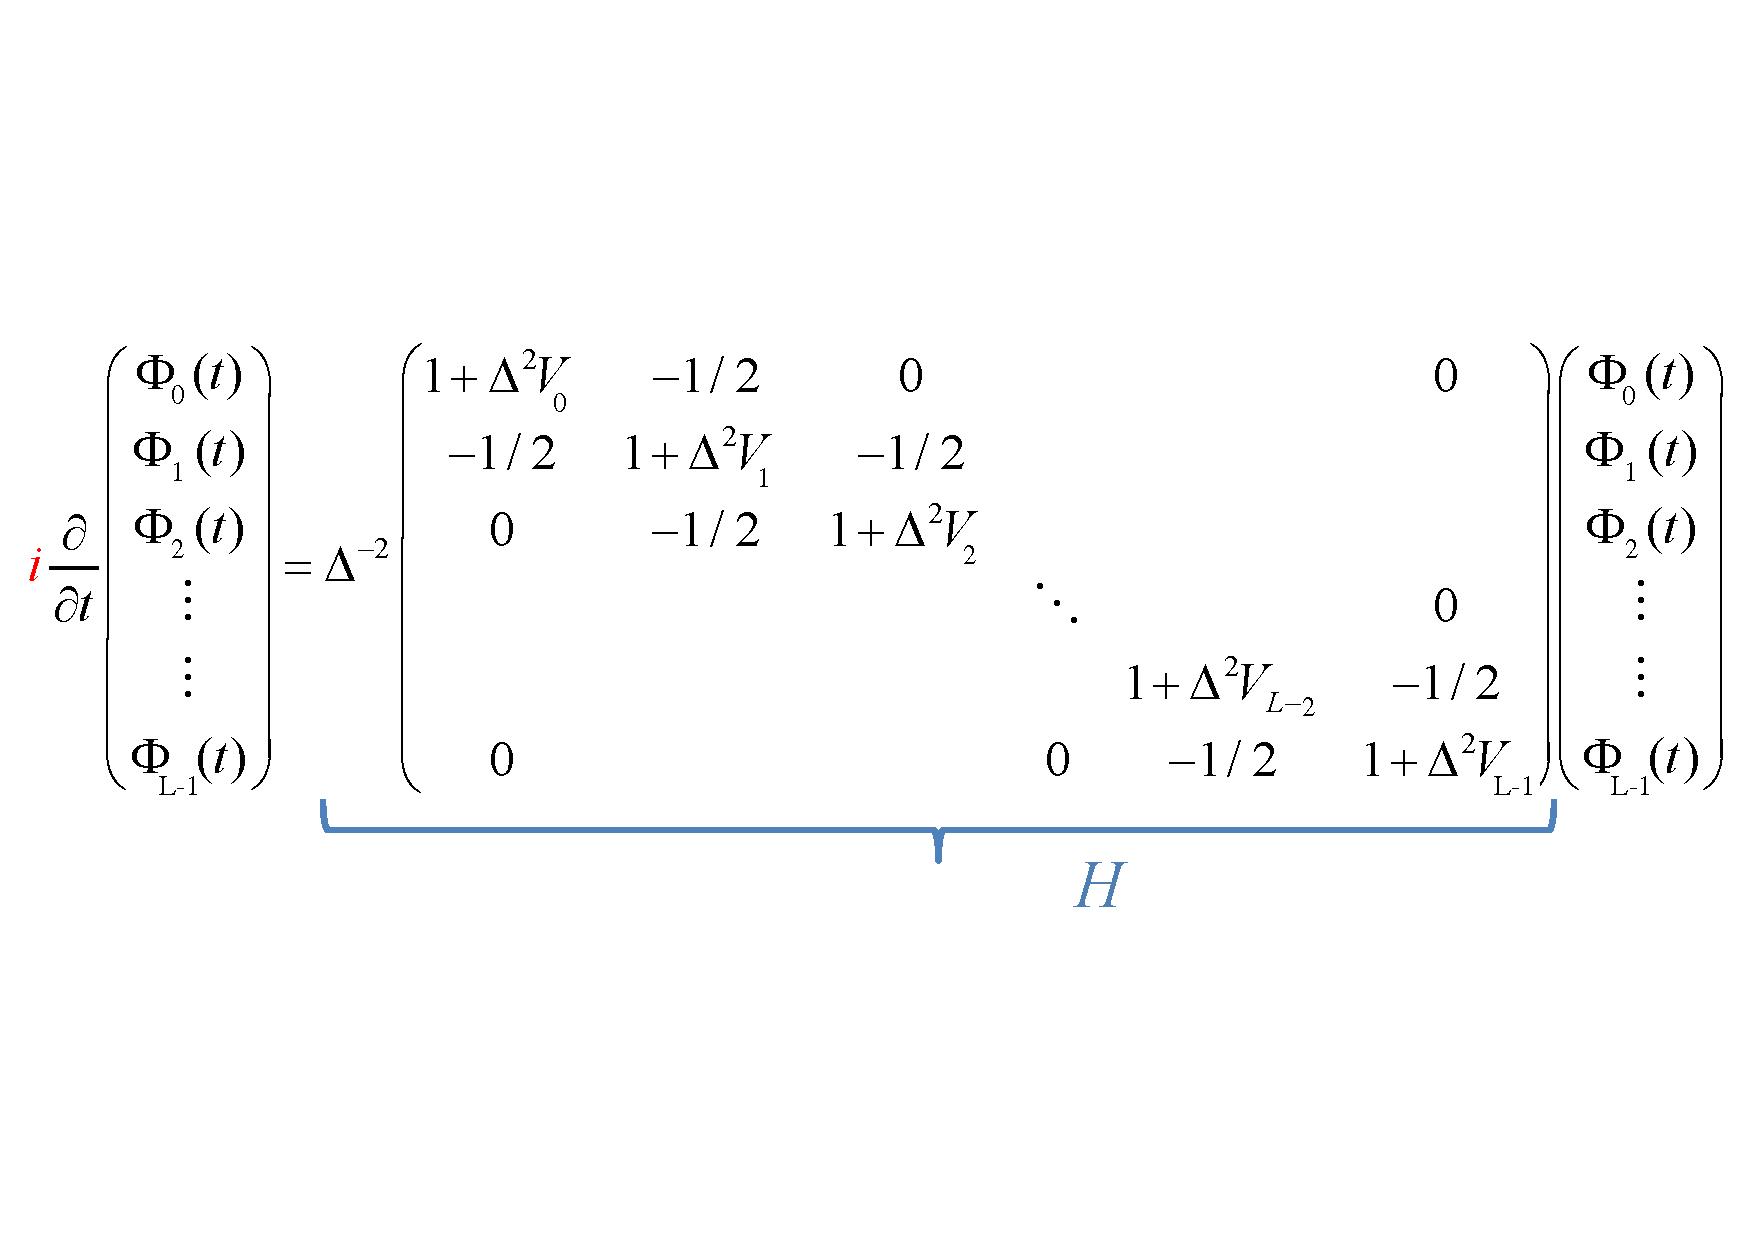
\includegraphics[width=.8 \textwidth]{Images/p39new.pdf}
\caption*{\tiny{source: Computational Physics - Lecture 17:
Time-dependent Schr\"odinger equation I (page 39)(edited)}}
\end{figure}

\noindent with $\Phi_i(t) = \Phi(x_i, t)$ and $V_i = V(x_i)$.

\noindent
The general solution for the Schr\"odinger equation is given by
\begin{equation}
    \Phi (x,t) = e^{-it\textcolor{NavyBlue}{H}}\Phi(x,t=0).
    \label{eq: gensol}
\end{equation}
Taking the exponential of $\textcolor{NavyBlue}{H}$ is cumbersome, which is why we resort to the use of second-order product formula approximation
\begin{equation}
     e^{-it \textcolor{NavyBlue}{H}}\approx \left(e^{-i\tau{K_1 \over 2}}e^{-i\tau{K_2 \over 2}} e^{-i\tau V}e^{-i\tau{K_2 \over 2}}e^{-i\tau{K_1 \over 2}}\right)^n = \left(e^{-i\tau \textcolor{NavyBlue}{H}}\right)^n.
     \label{eq: 2nd order}
\end{equation}
Our new task is to decompose $\textcolor{NavyBlue}{H}$, such that undertaking matrix exponentials is much easier. For that we decompose $\textcolor{NavyBlue}{H}$ into three different matrices $V,K_1,K_2$, such that
\begin{figure}[h!]
    \centering
    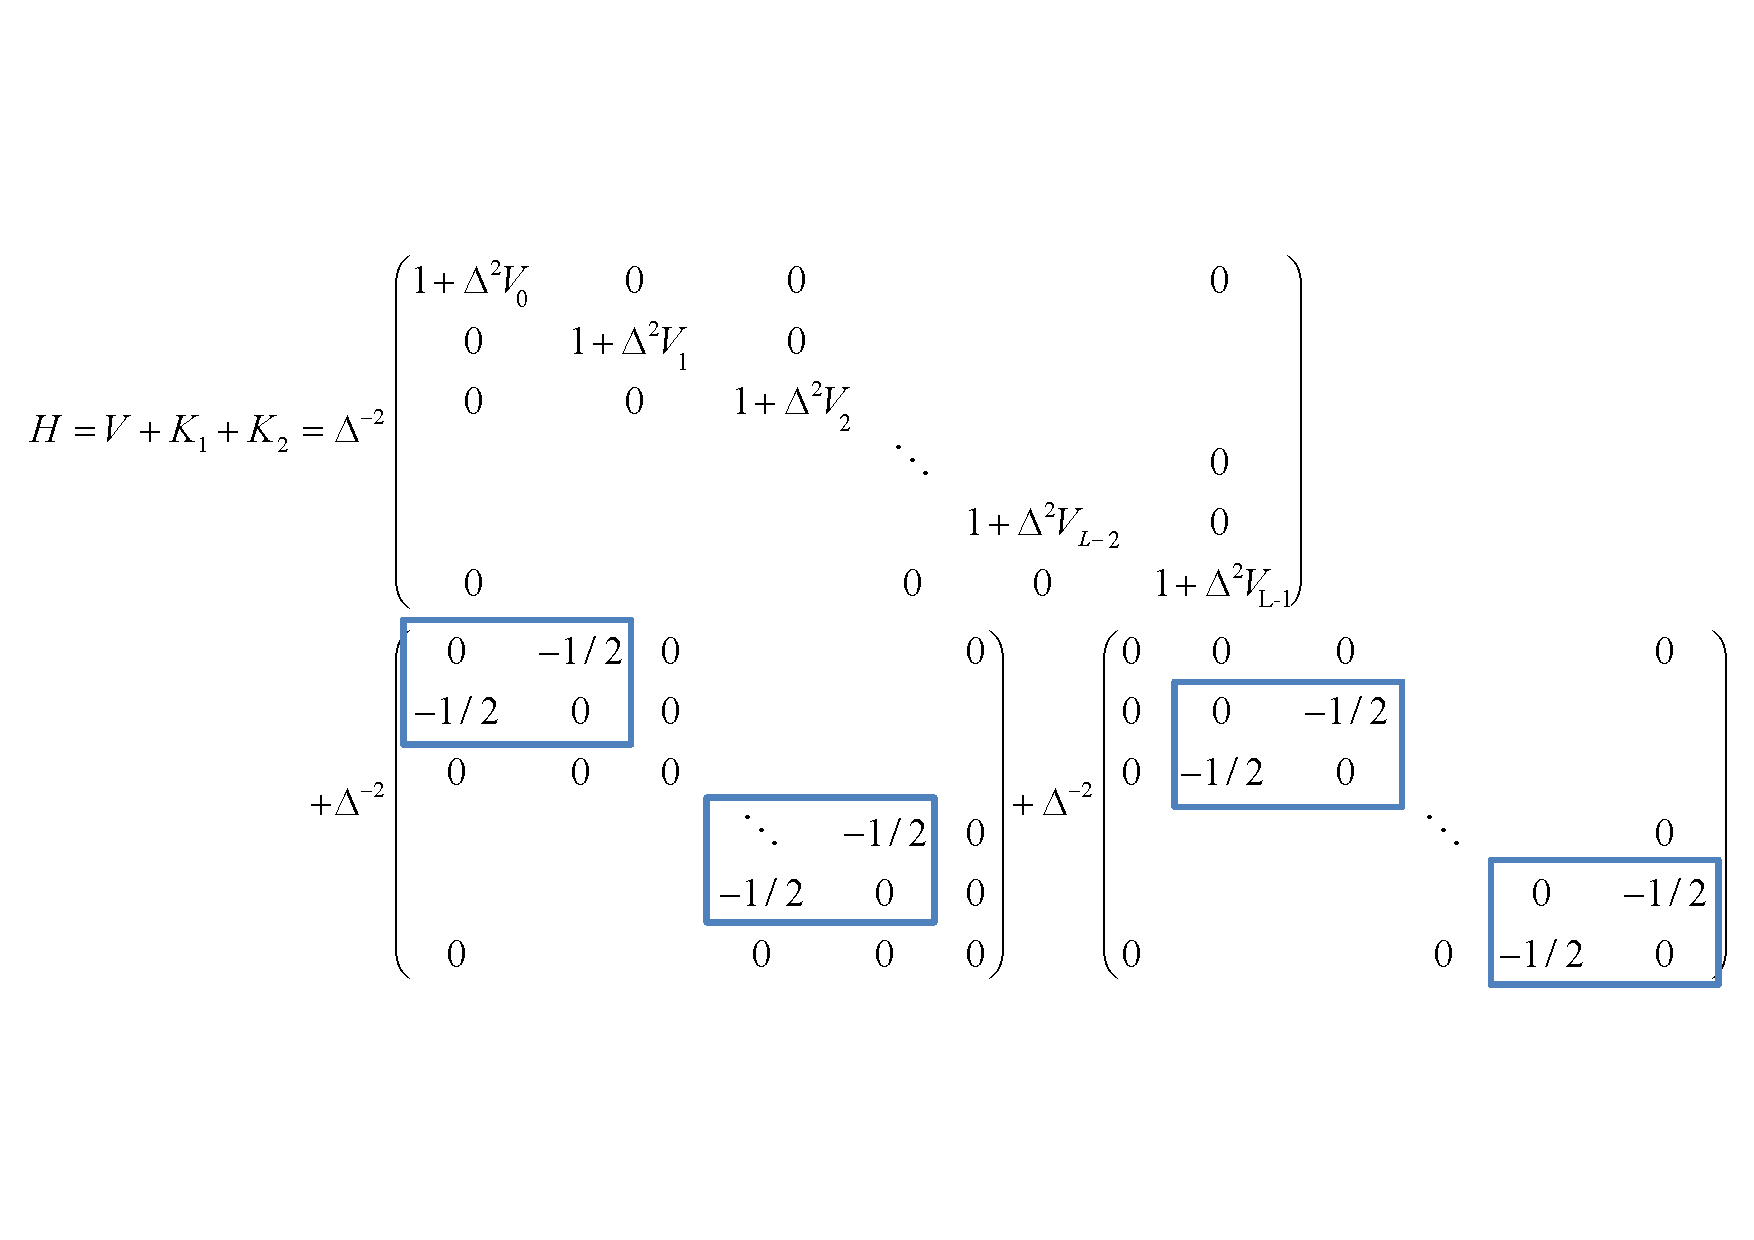
\includegraphics[width=.95 \textwidth]{Images/p49new.pdf}
\caption*{\tiny{source: Computational Physics - Lecture 17:
Time-dependent Schr\"odinger equation I (page 49)(edited)}}
\end{figure}
\clearpage
With the chosen decomposition, we see that the computation of $e^{-i\tau V}$ is very easy. It is a diagonal matrix with elements that are the exponentials of the diagonal elements. This is why calculating\footnote{$\Psi$ is an arbitrary array with the same dimensions as $\Phi$} 
\begin{align}
e^{-i\tau V}\Psi(x,t) &= \text{diag}(e^{-i\tau V_{00}},e^{-i\tau V_{11}},e^{-i\tau V_{22}},...,e^{-i\tau V_{(L-1)(L-1)}})\Psi(x,t)
\intertext{is done by }
e^{-i\tau V_{ii}}\Psi_i (t)&=\exp\left(-i\tau \underbrace{{1 \over \Delta ^2}(1+\Delta^2 V(x_i))}_{V_{ii}}\right)\Psi_i(t),
\label{eq: fynn}
\end{align}
with $i$ ranging from 0 to $L-1$. This corresponds to an elementwise multiplication of two arrays, which is implemented into \T{python} by creating an array consisting $\exp\left(-i \tau V_{ii}\right)$ at all positions $x_i$ and multiplying this with our array for $\Psi_i(t)$.\\

\noindent
For 
\begin{equation}
    e^{-i\frac{\tau}{2}{K_{1/2}}} \Psi(x,t),
\end{equation}
a different approach is chosen, due to the more complicated form of $K_{1/2}$.\footnote{$K_{1/2}$, which means either $K_1$ or $K_2$. } 
Fortunately, both $K_1$ and $K_2$ are composed of 2x2 matrices along the diagonal. Additionally, for $K_1$ the last entry is equal to zero, and for $K_2$, the first entry. To this end to multiply the matrices with $\Psi (x,t)$, we have to differentiate between the two cases
\begin{equation} 
\begin{split}
    &\exp \left(+ i{\tau\over 4\Delta^2 }
    \begin{pmatrix}
       0&1\\
       1&0\\
    \end{pmatrix}\right)
    \left(\begin{array}{c}
          \Phi _{k}(t)  \\
          \Phi _{k+1}(t)  \\
    \end{array}
    \right)\\ 
\end{split}
\end{equation}
and 
\begin{equation} \exp \left(+ i{\tau\over 4\Delta^2 }\cdot 0\right)
          \Phi(k,t) = \Phi(k,t).
          \label{eq: short}
\end{equation} 
It is easy to show that \refEq{eq: long} can be rewritten into
\begin{equation} 
    \exp \left(+ i{\tau\over 4\Delta^2 }
    \begin{pmatrix}
       0&1\\
       1&0\\
    \end{pmatrix}\right)
    \left(\begin{array}{c}
          \Phi _k (t)  \\
          \Phi _{k+1}(t)  \\
    \end{array}
    \right)
={\begin{pmatrix}
       \cos(a)&i \sin(a)\\
       i \sin(a)& \cos(a)\\
    \end{pmatrix}} \left(\begin{array}{c}
          \Phi _{k}(t)  \\
          \Phi _{k+1}(t)  \\
    \end{array}
    \right),
    \label{eq: long}
\end{equation}
with $a = {\tau\over 4\Delta^2 }$. With the last entry of $K_1$ being the zero entry, $k$ in \refEq{eq: long} must take all even numbers from $0$ to $L-2$. For $K_2$, the opposite is true, such that we have to take all the odd numbers from $1$ to $L-1$.\footnote{here, with $K_{1/2}$ we are referring to $e^{-i\tau{K_{1/2} \over 2}}$}$^,$\footnote{There is no need for an explicit implementation of \refEq{eq: short}, as doing no operation on an entry is the same as multiplying it by 1.}
The multiplication of a matrix with a vector is realized in \T{python} using \texttt{np.dot(a,b)}, which outputs the product of \T{a} and \T{b}. 
\clearpage
The index $k$ does not take all the numbers, but only the even ones for $K_1$ and the odd ones for $K_2$. To this end, choosing \texttt{for k in range(0,L-1,2)}, the counter \texttt{k} gets incremented by 2 in each step, such that with $k$ we have the even numbers and with $k+1$ the odd.

 In the code snippet below, we show the implementation of the function \T{dt(phi)}.
 Said function takes in a $\Phi (x,t)$ as an input and returns $\Phi (x,t+\tau)$, which is the wavefunction's evolution for one time step $\tau$. Calling this $n$ times iteratively, with the new input being the last output, results in the wavefunction at $t = n\tau$.\footnote{if the initial input was the $\Phi ({x,0})$}

\begin{lstlisting}[language=Python]
M    = np.array([[np.cos(a), 1j*np.sin(a)], [1j*np.sin(a), np.cos(a)]], dtype=np.complex128)  

def dt(phi):
    for k in range(0,len(phi)-1,2):             #K1
        phi[k:k+2] = np.dot(M,phi[k:k+2])
    for k in range(0,len(phi)-1,2):             #K2
        phi[k+1:k+3] = np.dot(M,phi[k+1:k+3])
    phi = Vx*phi                                #V part
    for k in range(0,len(phi)-1,2):             #K2
        phi[k+1:k+3] = np.dot(M,phi[k+1:k+3])
    for k in range(0,len(phi)-1,2):             #K1
        phi[k:k+2] = np.dot(M,phi[k:k+2])
    return phi
\end{lstlisting}

Using \T{phi[k:k+2]} (line 5 and 12 in code snippet), the vector $(\Phi_k,\Phi_{k+1})$ is sliced from the total array.\footnote{similar for the odd case (line 7 and 10 in code snippet)}\\

\noindent Apart from the wave function, we are interested in the probability density, defined as
\begin{equation}
P(x,t) = |\Phi(x,t)|^2 \quad \Rightarrow \quad  P(x_i,t) = |\Phi _i(t)|^2.\footnote{The absolute value can be calculated using \texttt{np.absolute()}.} \label{eq: P}	
\end{equation}


\noindent 
Next, we dedicate ourselves to the calculation of the mean position $\braket{x}$. According to \refEq{eq: scalar}, this is done by
\begin{align}
	\braket{x(t)} &= \Int{x|\Phi {(x,t)}|^2}.
\intertext{Due to the positions being discretized, we have }
x \rightarrow x_i, \qquad &|\Phi {(x,t)}|^2 \rightarrow |\Phi _i (t)|^2, \qquad dx \rightarrow \Delta \nonumber\\ 
\intertext{such that}
\braket{x_i(t)}&= \sum _{i = 0}^{L-1} x_i P(x_i,t) \Delta.\label{eq: x dis}
\intertext{Similarly, for $\braket{x^2}$ we have}
\braket{x_i^2(t)}&= \sum _{i = 0}^{L-1} x_i^2 P(x_i,t) \Delta.\label{eq: xx dis}
\end{align}
These two sums (\refEq{eq: x dis} and \refEq{eq: xx dis}), can be implemented into \T{python} using
\[
\braket{x_i(t)} = \T{np.sum(x*P*Delta)} \qquad \text{and} \qquad  \braket{x_i^2(t)} = \T{np.sum(x**2*P*Delta)},
\]
with $\T{P} = P(x_i,t)$. From there the variance can be calculated according to \refEq{eq: var} from \refEq{eq: x dis} and \refEq{eq: xx dis}:
\[
\text{Var}(x_i) = \braket{x_i^2(t)} - \braket{x_i(t)}^2.
\]
\section{Simulation results}
In this section, we present the solutions we obtained for the algorithm. To this end, we vary the parameters that affect the simulation. We study five different pairs for the parameters
\begin{equation}
(\Omega, \sigma, x_0) = (1,1,0),\ (1,1,1),\ (1,2,0),\ (2,1,1),\ (2,2,2)	.
\end{equation}
For the spatial discretization, we chose $\Delta = 0.025$ and $L = 1201$. For the discretization in time $\tau = 0.00025$ and $m = 40000$, such that the algorithm stops at $t = m\tau = 10$.
For the positions' averages and variances, we plotted the analytical expectation according to \refEq{eq: x sol} and \refEq{eq: xx sol} in the same plot.
The probability density functions $|\Phi|^2$, are plotted for $t\in [0,2,4,6,8,10]$. {As the Gaussian packet is localized in the vicinity of zero, we chose to plot $x$ from $-5$ to $5$.}
\begin{figure}[h!]
     \begin{subfigure}[h]{1\textwidth}
         \centering
         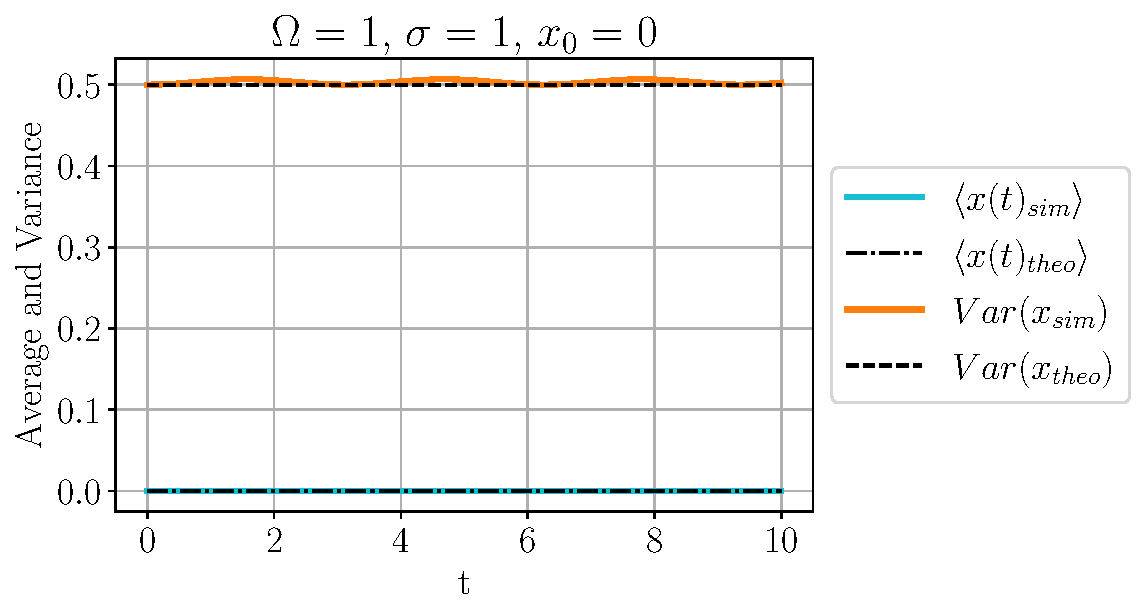
\includegraphics[width=\textwidth]{plot/Omega1_sigma1_x00_Averages.pdf}
         \caption{}
         
     \end{subfigure}
     \begin{subfigure}[h]{1\textwidth}
         \centering
         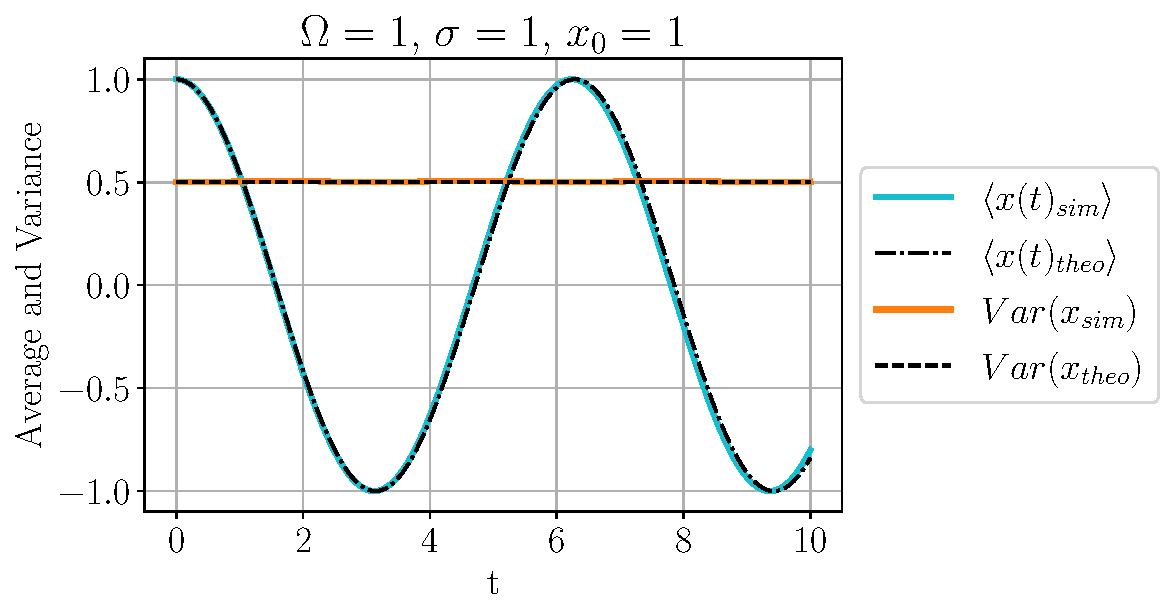
\includegraphics[width=\textwidth]{plot/Omega1_sigma1_x01_Averages.pdf}
         \caption{}
         
     \end{subfigure}
     \begin{subfigure}[h]{0.65\textwidth}
         \centering
         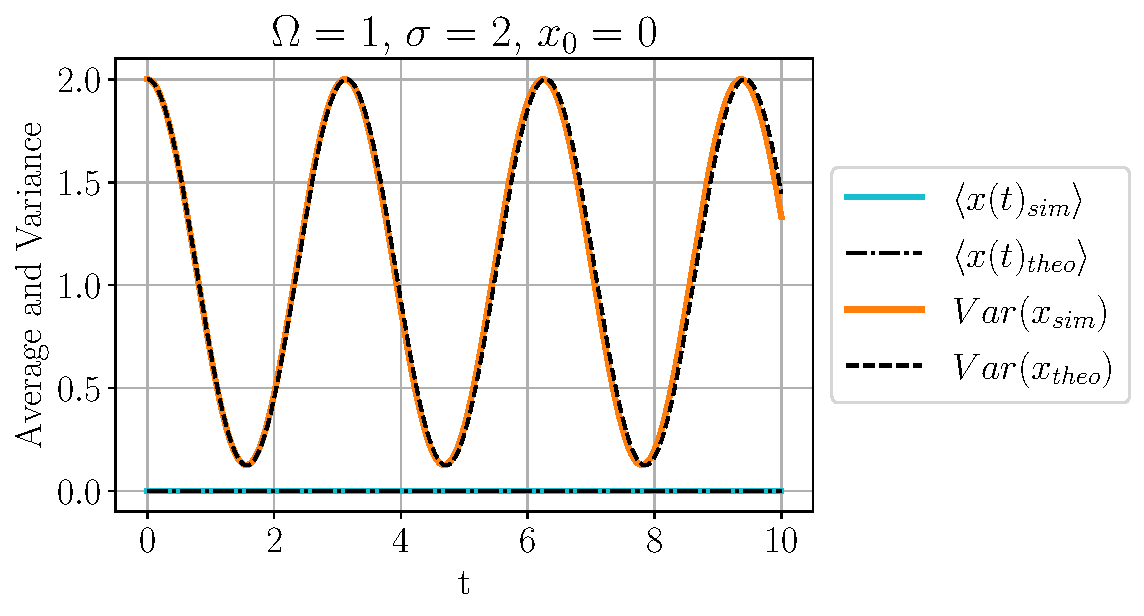
\includegraphics[width=\textwidth]{plot/Omega1_sigma2_x00_Averages.pdf}
         \caption{}
         
     \end{subfigure}
     \begin{subfigure}[h]{0.4\textwidth}
         \centering
         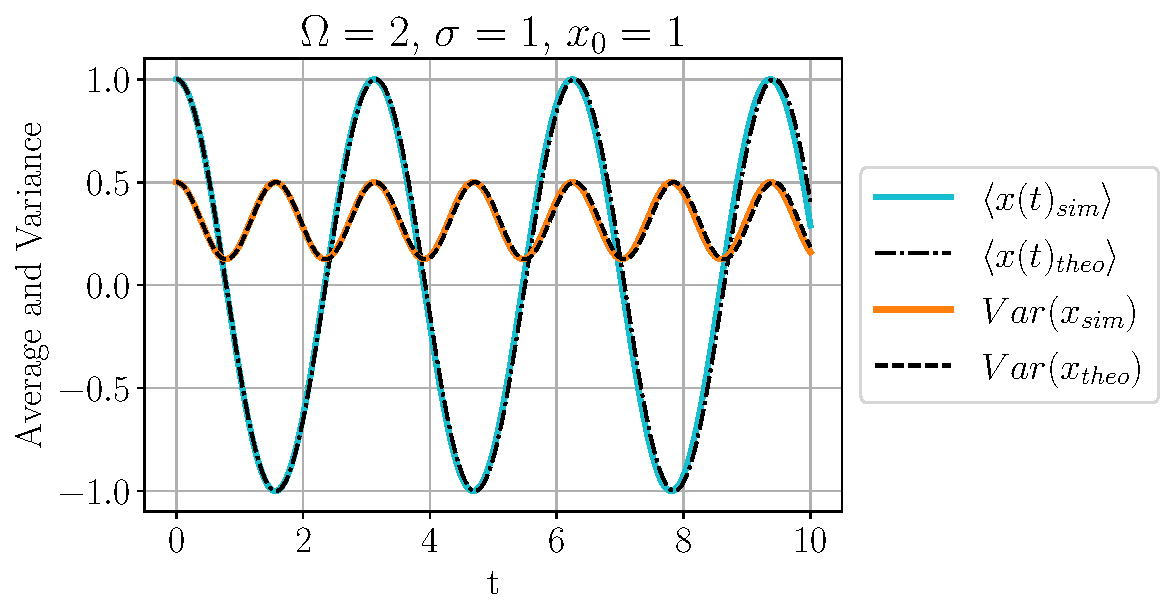
\includegraphics[width=\textwidth]{plot/Omega2_sigma1_x01_Averages.pdf}
         \caption{}
     \end{subfigure}
     \begin{subfigure}[h]{0.65\textwidth}
         \centering
         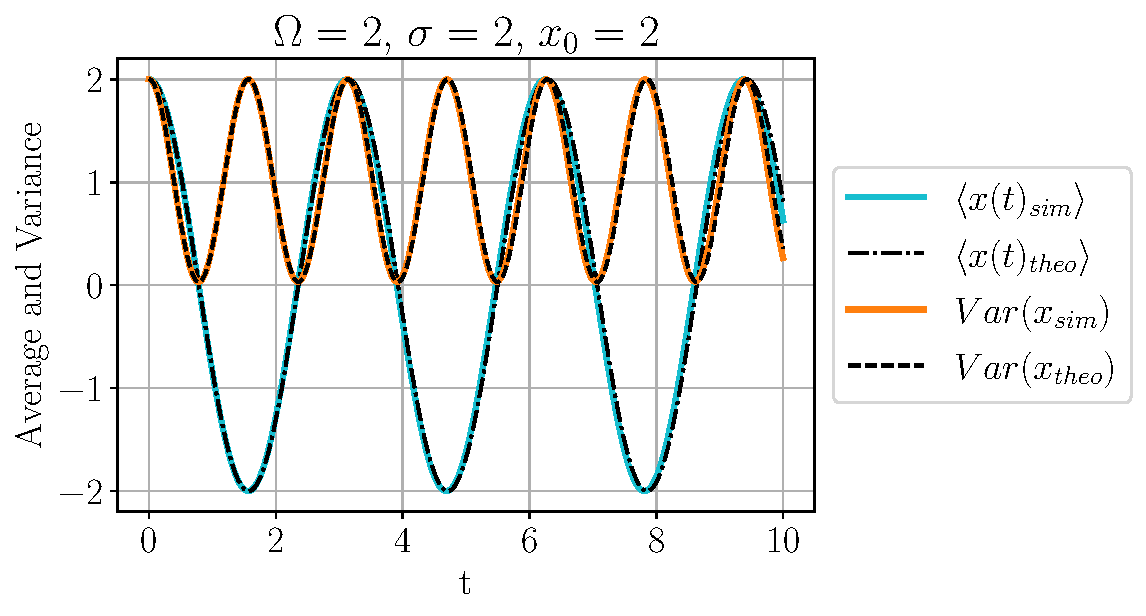
\includegraphics[width=\textwidth]{plot/Omega2_sigma2_x02_Averages.pdf}
         \caption{}
     \end{subfigure}
\caption{Simulation results for the average and variances for the position. In the title of each plot, the parameters $\Omega, \sigma$, and $x_0$ used are specified. The solid lines show the results according to the simulation model and the dashed line the theoretical expectation according to \refEq{eq: x sol} and \refEq{eq: xx sol}.}
\label{fig: Averages}
\end{figure}

\begin{figure}[h!]
     \begin{subfigure}[h]{0.65\textwidth}
         \centering
         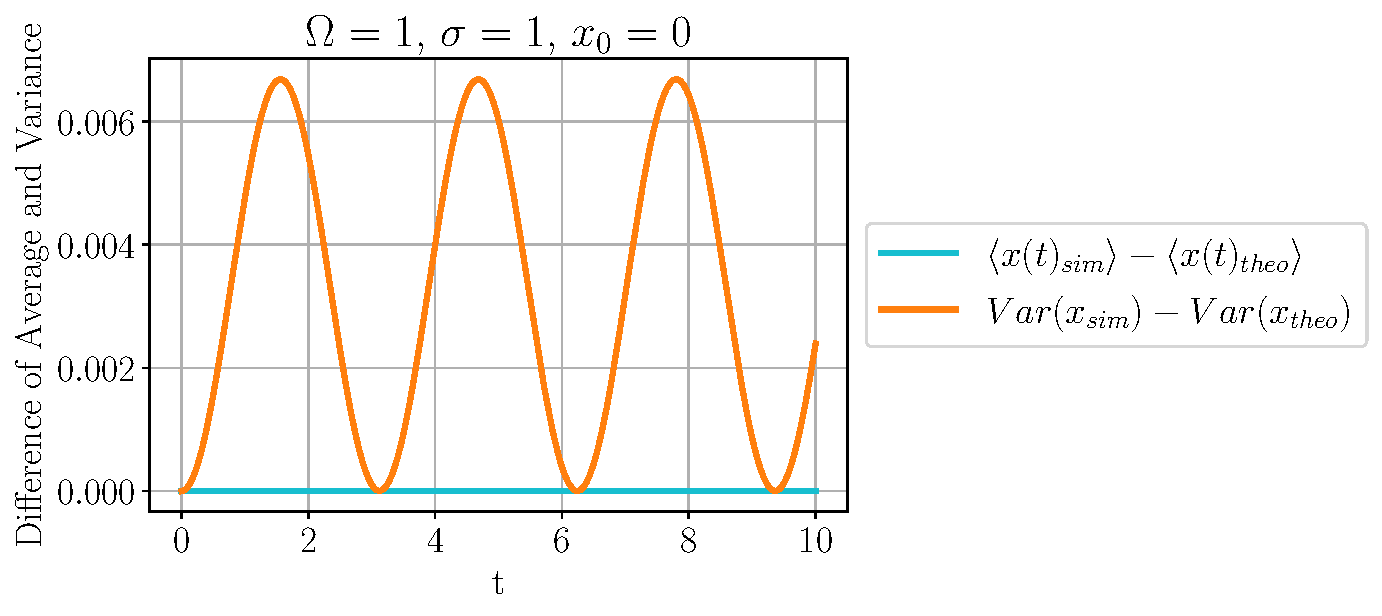
\includegraphics[width=\textwidth]{plot/Omega1_sigma1_x00_Averages_expect.pdf}
         \caption{}
         
     \end{subfigure}
     \begin{subfigure}[h]{0.4\textwidth}
         \centering
         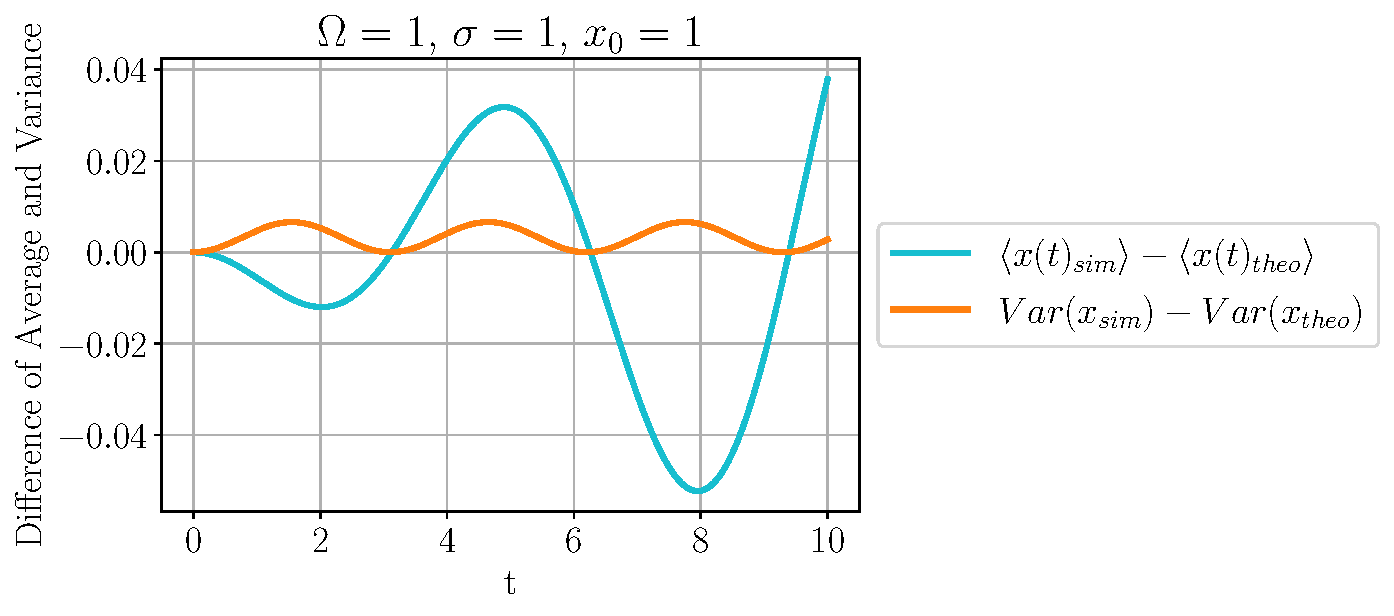
\includegraphics[width=\textwidth]{plot/Omega1_sigma1_x01_Averages_expect.pdf}
         \caption{}
         
     \end{subfigure}
     \begin{subfigure}[h]{0.65\textwidth}
         \centering
         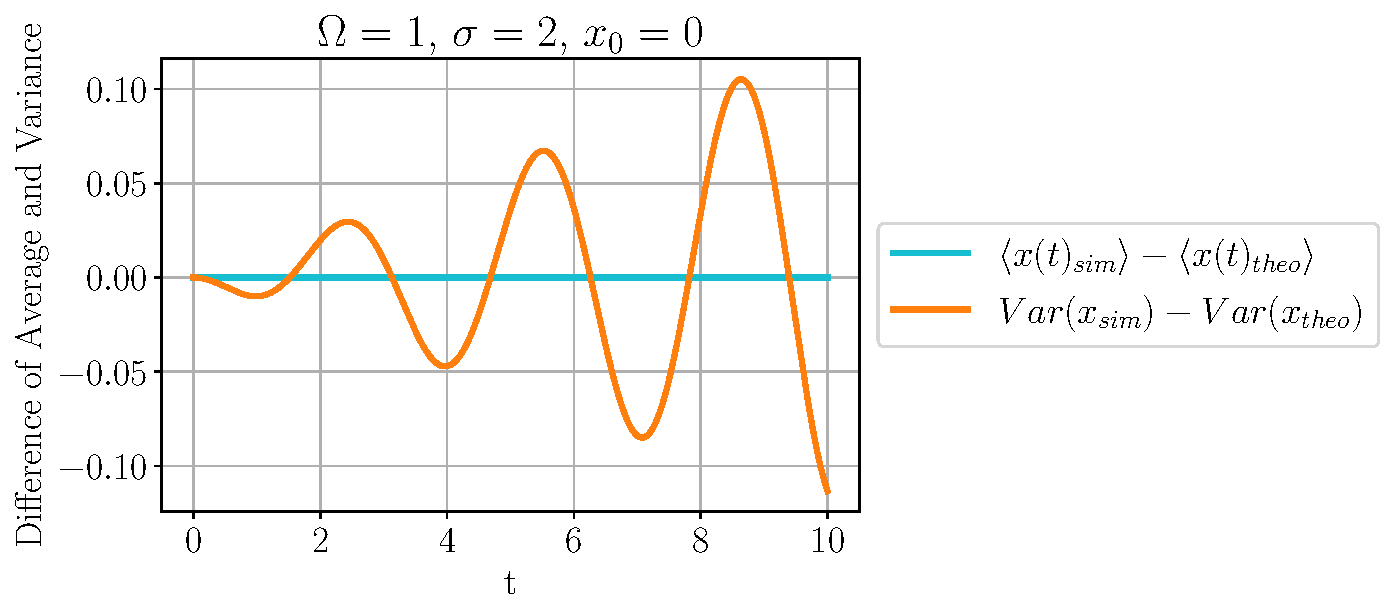
\includegraphics[width=\textwidth]{plot/Omega1_sigma2_x00_Averages_expect.pdf}
         \caption{}
         
     \end{subfigure}
     \begin{subfigure}[h]{0.4\textwidth}
         \centering
         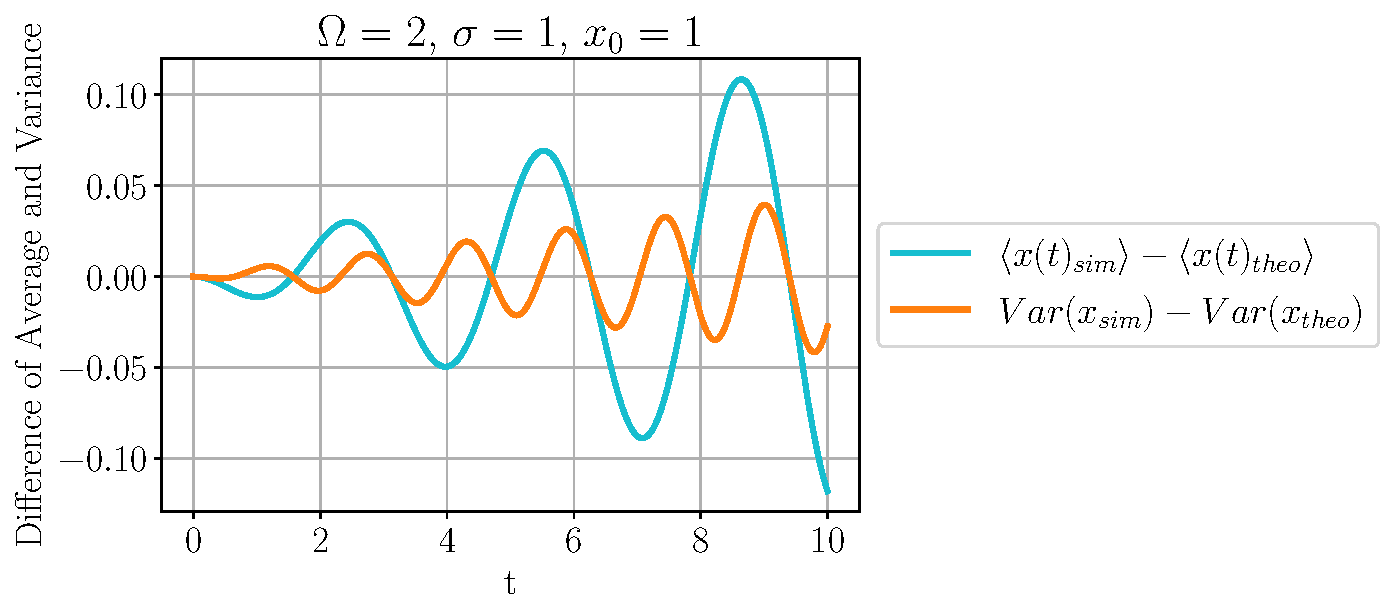
\includegraphics[width=\textwidth]{plot/Omega2_sigma1_x01_Averages_expect.pdf}
         \caption{}
     \end{subfigure}
     \begin{subfigure}[h]{0.65\textwidth}
         \centering
         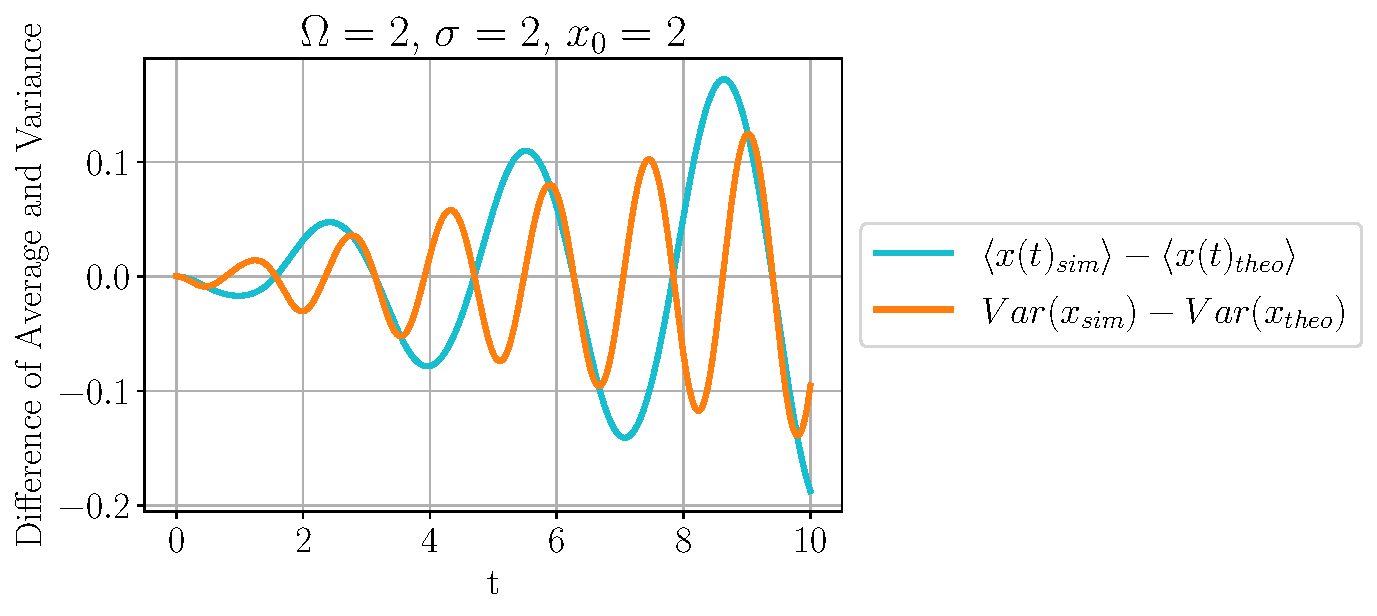
\includegraphics[width=\textwidth]{plot/Omega2_sigma2_x02_Averages_expect.pdf}
         \caption{}
     \end{subfigure}
\caption{Difference between simulation results and theoretical expectation for the average and variances for the position. In the title of each plot, the parameters $\Omega, \sigma$, and $x_0$ used are specified.}
\label{fig: difference}
\end{figure}



\begin{figure}[h!]
\centering
     \begin{subfigure}[h]{0.7\textwidth}
         \centering
         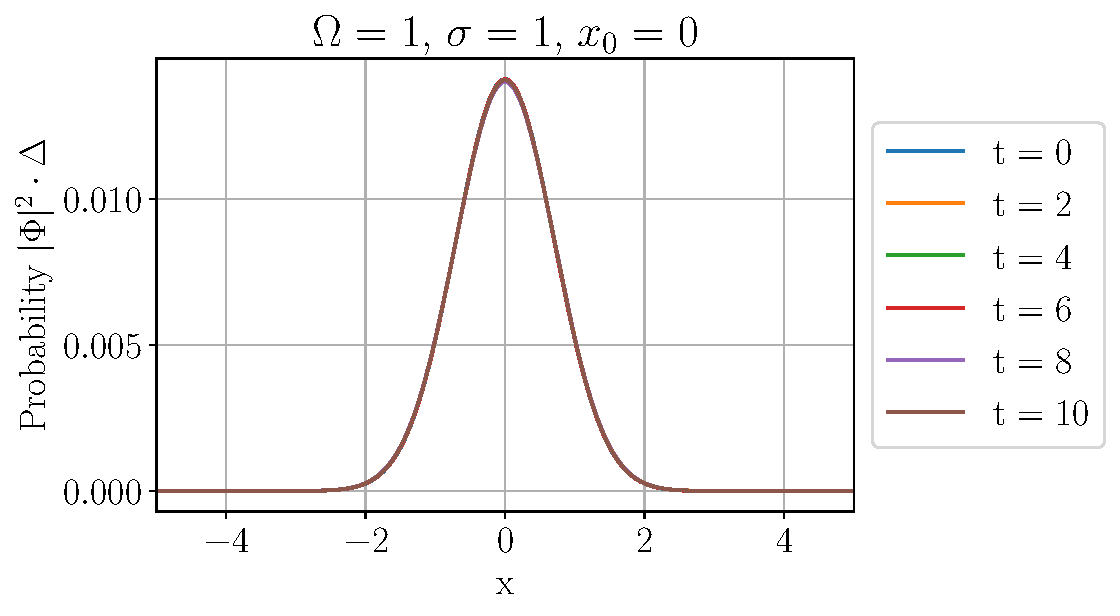
\includegraphics[width=\textwidth]{plot/Omega1_sigma1_x00_Probabilities.pdf}
         \caption{}
     \end{subfigure}

     \begin{subfigure}[h]{0.7\textwidth}
         \centering
         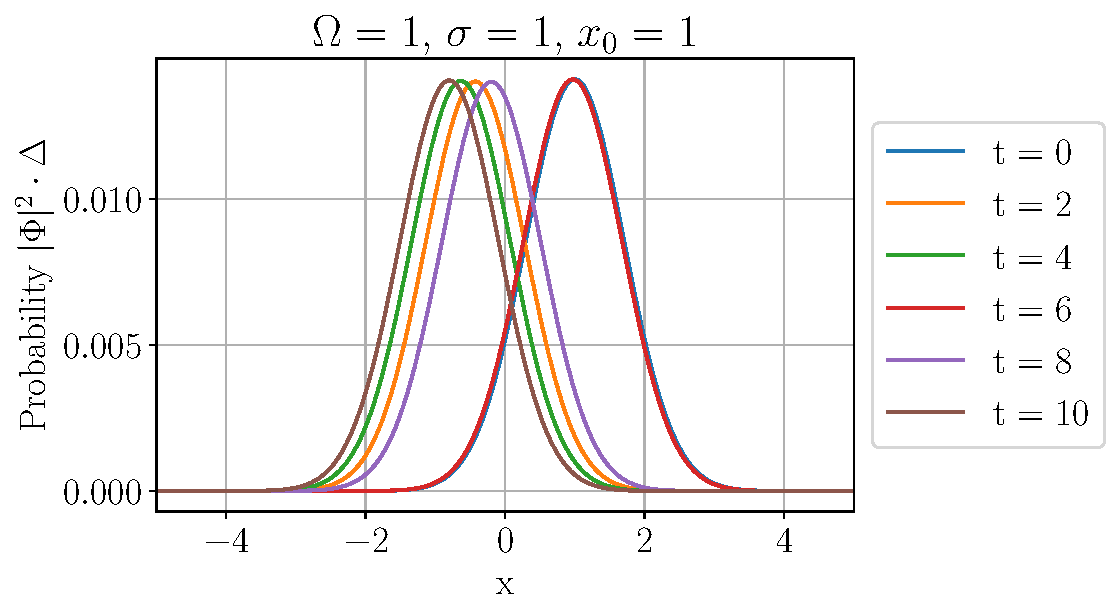
\includegraphics[width=\textwidth]{plot/Omega1_sigma1_x01_Probabilities.pdf}
         \caption{}
         
     \end{subfigure}
     
     \begin{subfigure}[h]{0.7\textwidth}
         \centering
         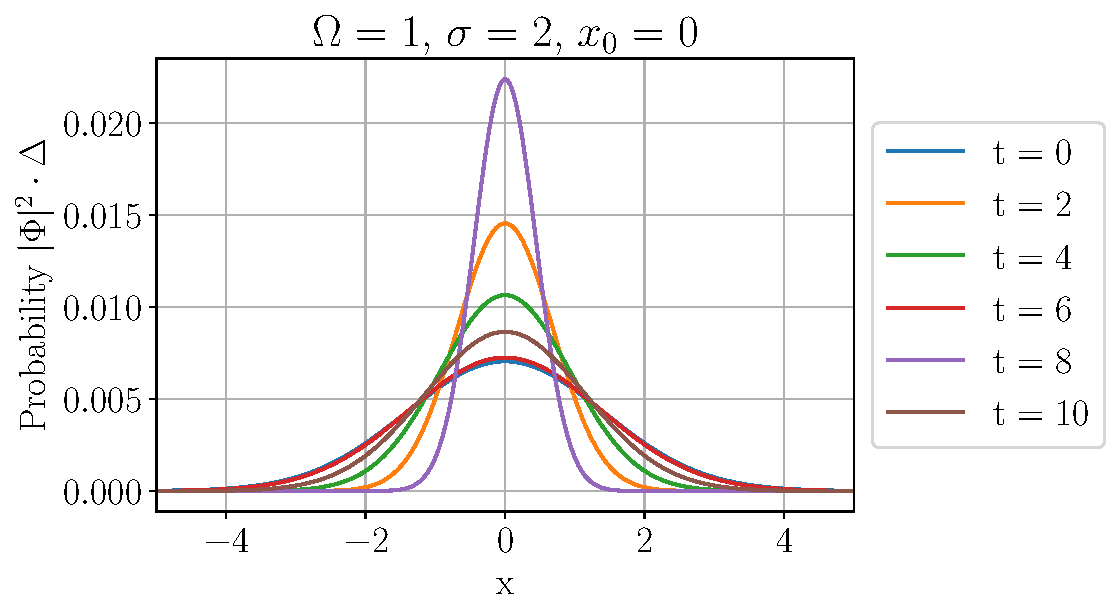
\includegraphics[width=\textwidth]{plot/Omega1_sigma2_x00_Probabilities.pdf}
         \caption{}
        
     \end{subfigure}
\end{figure}

\begin{figure}[h!]\ContinuedFloat
\centering
     \begin{subfigure}[h]{0.7\textwidth}
         \centering
         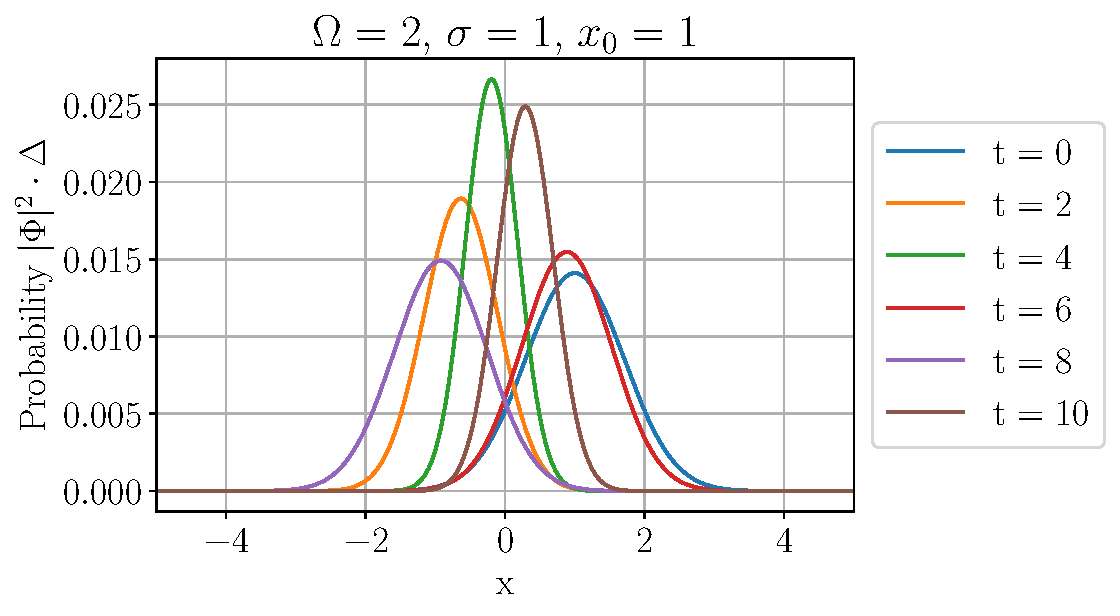
\includegraphics[width=\textwidth]{plot/Omega2_sigma1_x01_Probabilities.pdf}
         \caption{}
         
     \end{subfigure}
     
     \begin{subfigure}[h]{1\textwidth}
         \centering
         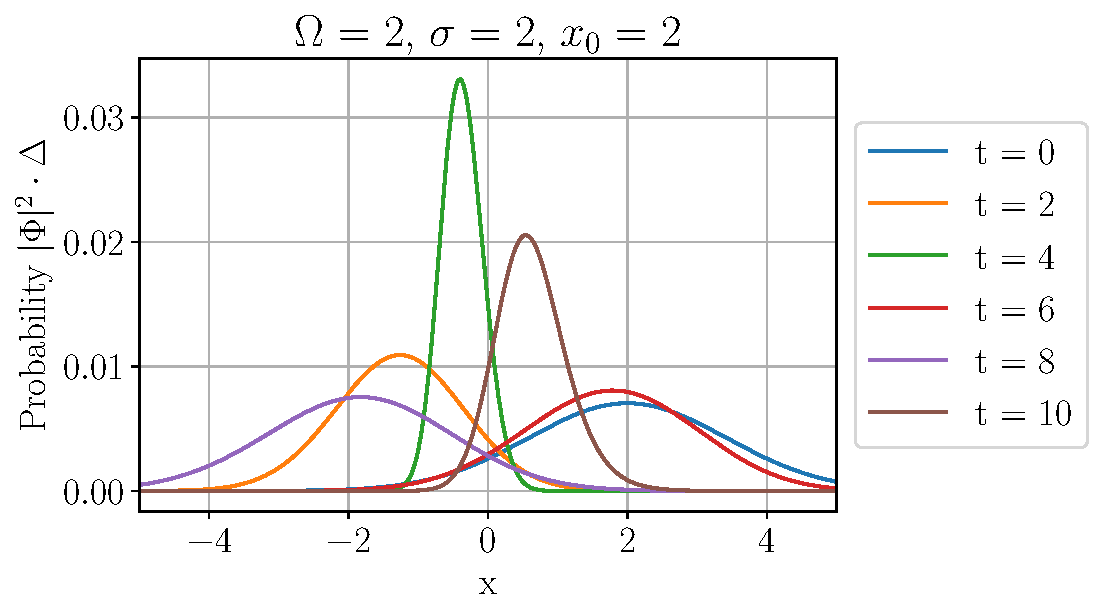
\includegraphics[width=\textwidth]{plot/Omega2_sigma2_x02_Probabilities.pdf}
         \caption{}
         
     \end{subfigure}
\caption{Simulation results for the Probabilities $|\Phi(x,t)|^2$. In the title of each plot, the parameters $\Omega, \sigma$, and $x_0$ used are specified. The functions are plotted for the six different times $t= 0,2,4,6,8,10$. The system is bounded to $-15 \leq x \leq 15$, but only $-5$ to $5$ is shown here.}
\label{fig: Probabilities}
\end{figure}


\clearpage
\section{Discussion}

We start the discussion by describing \refFig{fig: Probabilities}. To this end, we point out the main similarities and differences. (a) and (b) share the property that the probability function does not change its shape with time, i.e. the variance stays constant. In \refFig{fig: Averages} this becomes more obvious as the Variance in (a) and (b) stay constant at $1/2$ over time. However, it needs to be noted that the theoretical values do not exactly match with our simulation, this is not only restricted to (a) and (b) but to all the results. This, we investigate later. The reason why (a) and (b) are so different from the other cases is due to them being coherent states. While (a) depicts the scenario of the vacuum state itself, (b) describes a coherent state with non-zero $\alpha$.\footnote{$\alpha$ depicts the amplitude and phase of a coherent state} The interesting property of coherent states is that they resemble classical behavior. Imagine a ball in the classical harmonic oscillator. If the initial position of the ball is at the minimum, we do not expect anything to happen with the ball. This is analogous to our case (a). If, however, the ball is slightly displaced from the minimum, the ball starts to oscillate to the left and right, similar to our case (b). Additionally, the fact that the wave function is preserving its shape, is because coherent states stay coherent in the quantum harmonic oscillator. This in particular is very interesting, as these states are not eigenstates of our Hamiltonian. In (c), the behavior is striking, as it is the only case, where the average position stays constant, that is at 0, but the variance oscillates over time. The frequency at which the variance oscillates is $2\Omega$. Also, the difference between (a) and (c) is only the $\sigma$, but contrary to (a) the variance oscillates. This is due to \refEq{eq: xx sol}, where for $\Omega,\sigma = 1$, the variance is equal to a constant. But there is an underlying relation between $\Omega$ and $\sigma$, that governs the cases when the variance does not change over time. This relation can be derived from \refEq{eq: xx sol} when the constants in front of the $\sin^2(\Omega t)$ and $\cos^2(\Omega t)$ are the same, or simply put
\begin{equation}
	{1\over \sigma^2 \Omega^2} = \sigma^2 \quad \rightarrow \quad \Omega \sigma^2 = 1.
\end{equation}
We can see that our initial conditions for (a), satisfy this relation.\\

Considering (d) and (e), we see they are very similar. In both cases, we have a wave packet that is initially displaced from 0, which is why it oscillates back and forth. While (d) starts at $x_0 = 1$, (e) starts at $x_0 = 2$. Comparing the average positions in \refFig{fig: Averages} for both (d) and (e), one sees that in both cases the frequency is the same. This was also shown in the theoretical derivation (see \refEq{eq: x sol}), that the frequency of the average does only depend on $\Omega$. This behavior matches our expectations from classical mechanics. Independent of the location of the ball, it oscillates with the same frequency. Other than the mean position being the actual position of the ball, there is no difference in the solution for the position. Turning to the variances of (d) and (e), one can see that similar to (c), how it oscillates too. However, for (d) and (e) $\Omega$ was chosen twice as large as in (c), which is why the variance oscillates with double the frequency of (c). The difference between (d) and (e) is, that for choosing a larger $\sigma$, the amplitude of the variance oscillation is larger.\\

After having discussed the simulation results and comparing them with each other, we turn to the theoretical expectation. In \refFig{fig: Averages}, additionally to our simulation the theoretical results derived in section \ref{sec: theo} are plotted as the dashed line. In (a), we can see how the theoretical expectation for $\braket{x(t)}$ matches the results very well. However, for the variance, it seems like our simulation oscillates above the expectation. These are probably artifacts due to discretizations and approximations, as we have seen similar behavior in the exercise about "Molecular Dynamics Simulation". For further investigation, \refFig{fig: difference} shows the differences between the simulation and theoretical result. Here, our hypothesis of oscillation above the theoretical expectation is proved to be true. Interestingly, the oscillation frequency coincides with the frequency $\Omega$. In (b), similar to (a), the variance oscillates although again the theoretical expectation should be constant. But in both (a) and (b), it seems that the amplitude of the oscillation does not change over time. For (c), (d), and (e), the difference between simulation and theory, oscillates, but the amplitude increases gradually. For the mean position, we have similar behavior. In (b), (d), and (e), the difference oscillates, and at the same time the amplitude increases. Only for (a) and (c), the difference stays constant and is equal to 0. But these are the cases in which the position does not change at all, which is why we can deduct that the $x_0 = 0$ cancels the error that is responsible for the difference. As the theory predicts $x_0 \cos(\Omega t)$, we expect that the error lies in the frequency $\Omega$ such that our simulation does not fully compute the exact $\cos (\Omega t)$, but a small deviation $\cos (\Omega '(t) t)$ from that. This deviation of the true frequency is likely time-dependent. Similar reasoning is also expected for the variances. It has probably to do with the second-order product formula only being an approximation.\\

Overall one can summarize that the simulation method using the second-order product formula and discretizing the system yields results that are in good reasoning with the theory. However, it needs to be pointed out that any approximation is only an approximation which is why deviations will increase with more and more iterations. Additionally, numerical uncertainties are also a source of errors. Nevertheless, the method used is very viable to produce good results. The advantage of this simulation is how versatile it is, changing the initial condition or parameters can be done easily, whereas doing it analytically would take much more time.



\clearpage
\appendix
\section{Code}

In the section about the simulation model, the use of multiprocessing was not discussed. As this only makes the code more efficient, it was of no avail to explain it there. The basic idea is to calculate the same function with different arguments parallel. This has the advantage that the runtime is reduced drastically for five different inputs.


%TODO comment on code


\begin{lstlisting}[language=Python]
#!/usr/bin/env python3
# -*- coding: utf-8 -*-
"""
Created on Fri Jul 14 15:46:58 2023

@author: tamilarasan
"""
import numpy as np
import matplotlib.pyplot as plt
from numba import njit, vectorize, float64
import time

start = time.time()
from multiprocessing import Pool
import os 
os.environ["PATH"] += os.pathsep + '/Library/TeX/texbin'

plt.rcParams["text.usetex"] = True
plt.rcParams["font.family"] = "times new roman"
plt.rcParams["font.size"] = "18"

pi      = np.pi  



Delta = 0.025
L = 1201
tau = 0.00025
m = 40000


def solve(Input): 
    Omega, sigma, x0 = Input
    
    c = np.cos(tau/(4*Delta**2))
    s = 1j*np.sin(tau/(4*Delta**2))
    M = np.array([[c,s],[s,c]], dtype=np.complex128) 
    
    x = np.linspace(-15,15,L)
    @njit
    def Phi0(x):
        return (pi*sigma**2)**(-1/4)*np.exp(-(x-x0)**2/(2*sigma**2))
    
    Phi = np.array(Phi0(x)).astype(np.complex128) 
    
    @njit
    def V(x):
        return 1/2*Omega**2*x**2
    
    Vvec= np.vectorize(V)    
    Vx = np.exp(-1j*tau*(Delta**(-2)+Vvec(x)))
    
    @njit
    def dt(phi):
        for k in range(0,len(phi)-1,2):             #K1
            phi[k:k+2] = np.dot(M,phi[k:k+2])
        for k in range(0,len(phi)-1,2):             #K2
            phi[k+1:k+3] = np.dot(M,phi[k+1:k+3])
        phi = Vx*phi                                #V part
        for k in range(0,len(phi)-1,2):             #K2
            phi[k+1:k+3] = np.dot(M,phi[k+1:k+3])
        for k in range(0,len(phi)-1,2):             #K1
            phi[k:k+2] = np.dot(M,phi[k:k+2])
        return phi
    
    X = np.zeros(m+1)
    Xsq = np.zeros(m+1)
    tprint = [0,2,4,6,8,10]
    Pt = []
    for i in range(m):
        P = np.abs(Phi)**2
        if round(i*tau,5) in tprint:
            Pt+= [P]
        X[i] = np.sum(x*P*Delta)
        Xsq[i] = np.sum(x**2*P*Delta)
        Phi = dt(Phi)
    P = np.abs(Phi)**2
    Pt += [P]
    X[m] = np.sum(x*P*Delta)
    Xsq[m] = np.sum(x**2*P*Delta)
    plt.show()
    return X,Xsq,Pt


    

def plot(task,arg):
    Omega, sigma, x0 = arg
    legend = [[1,1,0],[1,2,0],[2,2,2]]
    X,Xsq,P = task
    t = np.linspace(0,m*tau,m+1)
    x = np.linspace(-15,15,L)
    xth = x0*np.cos(Omega*t)
    xsqth = 1/(2*Omega**2*sigma**2)*(np.sin(Omega*t))**2+ 1/2*(sigma**2+2*x0**2)*(np.cos(Omega*t))**2
    tprint = [0,2,4,6,8,10]
    
    plt.grid()
    plt.plot(t, X, label =r"Simulation $\langle x(t) \rangle$", color ="tab:blue")
    plt.plot(t, xth, label = r"Theory $\langle x(t) \rangle$", color = "tab:blue", ls = "--",alpha = 0.5)
    plt.plot(t, Xsq-X**2,label =r"Simulation $\langle x(t)^2 \rangle-\langle x(t) \rangle^2$", color ="tab:orange")
    plt.plot(t, xsqth-xth**2, label = r"Theory $\langle x(t)^2 \rangle-\langle x(t) \rangle^2$",alpha = 0.5, color = "tab:orange",ls = "--")
    plt.xlabel("t")
    plt.ylabel("Average and Variance")
    plt.title(r"$\Omega$ = "+str(Omega)+r", $\sigma$ = "+str(sigma)+r", $x_0$ = "+str(x0))
    if arg in legend:
        plt.legend(loc='center left', bbox_to_anchor=(1, 0.5))
    plt.savefig(f"plot/Omega{Omega}_sigma{sigma}_x0{x0}_Averages.pdf",bbox_inches='tight')
    plt.show()
    
    
    plt.grid()
    plt.plot(t, X-xth, label = r"$\langle x(t)_{sim} \rangle - \langle x(t)_{theo} \rangle$", color = "tab:blue")
    plt.plot(t, Xsq-X**2 - (xsqth-xth**2),label =r"$Var(x_{sim}) -Var(x_{theo})$", color ="tab:orange")
    plt.xlabel("t")
    plt.ylabel("Difference of Average and Variance")
    plt.title(r"$\Omega$ = "+str(Omega)+r", $\sigma$ = "+str(sigma)+r", $x_0$ = "+str(x0))
    if arg in legend:
        plt.legend(loc='center left', bbox_to_anchor=(1, 0.5))
    plt.savefig(f"plot/Omega{Omega}_sigma{sigma}_x0{x0}_Averages_expect.pdf",bbox_inches='tight')
    plt.show()
    
    for i in range(6):
        np.save(f"Data/tami_t{tprint[i]}_params{Omega}{sigma}{x0}.npy", P[i])
        plt.plot(x,P[i], label = "t = "+str(tprint[i]))
    plt.title(r"$\Omega$ = "+str(Omega)+r", $\sigma$ = "+str(sigma)+r", $x_0$ = "+str(x0))
    plt.xlabel("x")
    plt.xlim(-5,5)
    plt.grid()
    plt.ylabel("Probability")
    plt.legend(loc='center left', bbox_to_anchor=(1, 0.5))
    plt.savefig(f"plot/Omega{Omega}_sigma{sigma}_x0{x0}_Probabilities.pdf",bbox_inches='tight')
    plt.show()
    return 0

if __name__ == '__main__':
    pool = Pool()
    args = [[1,1,0],[1,1,1],[1,2,0],[2,1,1],[2,2,2]]
    Sol = pool.map(solve, args)

    for i in range(5):
        plot(Sol[i],args[i])


end = time.time()
print(end - start)
\end{lstlisting}







\end{document}
